\documentclass[conference]{IEEEtran}
\IEEEoverridecommandlockouts

\usepackage{cite}
\usepackage{amsmath,amssymb,amsfonts}
\usepackage{graphicx}
\usepackage{textcomp}
\usepackage{xcolor}
\usepackage{booktabs}
\usepackage{multirow}
\usepackage{url}

\def\BibTeX{{\rm B\kern-.05em{\sc i\kern-.025em b}\kern-.08em
    T\kern-.1667em\lower.7ex\hbox{E}\kern-.125emX}}
\begin{document}

\title{Apparent Inefficiency, Hidden Optimality: Why the Brain's Multimodal Attention Does Not Track Feature Strength}

\author{\IEEEauthorblockN{Anonymous}
\IEEEauthorblockA{
Paper ID: XXXX\\
Submitted for blind review}
}

\maketitle

\begin{abstract}
How does the brain allocate attention across sensory modalities during multimodal integration? Classical Bayesian frameworks predict that efficient systems weight each modality in proportion to its encoding strength. We tested this prediction using fMRI data from four participants watching naturalistic movies (~65 hours). Through unimodal encoding models and a personalized multimodal neural network with learnable modality weights, we found a striking dissociation: visual features dominated encoding (mean $r = 0.204$, 91\% of brain regions), yet the learned attention weights remained balanced ($\sim$33\% per modality). We term this the Encoding-Attention Dissociation. Critically, this finding was robust across multiple control analyses: it persisted when restricting analysis to high-encoding brain regions ($r > 0.2$, 407 regions), when using end-to-end training, and when substituting alternative feature extraction models (CLIP, Wav2Vec2, GPT-2). The Default Mode Network emerged as the primary integration hub (Multimodal Integration Index = 0.744), and hierarchical clustering confirmed that integration follows a gradient from modality-specific sensory regions to transmodal association cortex. These results suggest that the brain's multimodal integration strategy prioritizes robustness over narrow efficiency, maintaining balanced attention regardless of encoding strength.
\end{abstract}

\begin{IEEEkeywords}
multimodal integration, encoding models, attention allocation, fMRI, Default Mode Network, robust optimization
\end{IEEEkeywords}

\section{Introduction}

Multimodal integration is central to human cognition, enabling us to effortlessly understand naturalistic environments by binding visual, auditory, and linguistic information. How the brain achieves this integration---and how it allocates attentional resources across modalities---remains a fundamental question in computational neuroscience \cite{stein1993merging, beauchamp2004unraveling}.

A foundational view holds that the brain integrates multisensory signals in a statistically optimal manner, weighting each source according to its reliability \cite{ernst2002humans, knill2004bayesian}. This Bayesian framework predicts that stronger or less noisy signals receive proportionally greater attention during integration, as confirmed in visual-haptic \cite{ernst2002humans} and visual-vestibular \cite{fetsch2013bridging} integration. However, this efficiency principle may not hold universally. Under bimodal attention allocation, cross-modal balanced attention can enhance overall performance compared to focusing on a single channel \cite{mishra2012attention}. These findings suggest that the brain's attentional strategy may be more nuanced than a simple proportional weighting of each channel's reliability.

Encoding models provide a quantitative framework for linking stimulus features to brain activity \cite{naselaris2011encoding}. Previous work has demonstrated that deep neural network hierarchies correspond to visual processing hierarchies \cite{gucclu2015deep}, that language representations are distributed across cortex in organized gradients \cite{huth2016natural}, and that large language model representations predict brain activity during language processing \cite{caucheteux2022brains}. Building on these foundations, we employ encoding models to quantify modality-specific processing and test how the brain allocates attention across modalities.

The human cerebral cortex is organized hierarchically from primary sensory regions to higher-order association areas \cite{margulies2016situating}, formalized in the Schaefer parcellation with seven functional networks spanning unimodal to transmodal processing \cite{schaefer2018local}. The Default Mode Network (DMN) occupies a unique position in this hierarchy, implicated in semantic integration, narrative comprehension, and mental simulation \cite{mar2011neural, simony2016dynamic}. This hierarchical organization motivates the question: does the transition from unimodal to multimodal processing follow a systematic gradient, and where does the brain implement multimodal attention allocation?

We propose and test three hypotheses about multisensory processing. First, modality-specific encoding in early sensory regions gives way to shared, amodal representations in higher-order cortices. Second, integration follows a hierarchical structure with the DMN serving as a primary integration hub. Third, and most critically, attention allocation during multisensory integration is decoupled from encoding strength---a principle we term the \textit{Encoding-Attention Dissociation}. While the first two hypotheses are grounded in established findings about cortical hierarchy \cite{margulies2016situating} and serve as validation for our analytical framework, the novel contribution of this work lies in the third hypothesis and the extensive control analyses that establish its robustness.

\section{Methods}

\subsection{Data and Participants}

Functional MRI data were obtained from the Algonauts 2025 Challenge \cite{gifford2024algonauts}, derived from the Courtois NeuroMod project \cite{boyle2023courtois}. Four healthy adult participants viewed approximately 65 hours of movie content including the television series \textit{Friends} (seasons 1--6, 55 hours) for model training and validation (80\%/20\% split) and the Movie10 dataset (10 hours) as an independent test set. The fMRI data were acquired with a repetition time (TR) of 1.49\,s and parcellated into 1,000 cortical regions using the Schaefer atlas \cite{schaefer2018local}, which organizes the cortex into seven functional networks: Visual, Somatomotor, Dorsal Attention, Ventral Attention, Limbic, Frontoparietal, and Default Mode.

\subsection{Feature Extraction}

To extract stimulus representations, we employed one primary and one alternative model per modality to ensure findings generalize beyond any single feature extractor (see Section~\ref{sec:multimodel}). The primary models were: visual features from SlowFast 3D ResNet pretrained on Kinetics-400 \cite{feichtenhofer2019slowfast} (8,192 dimensions); auditory features from 20-dimensional mel-frequency cepstral coefficients (MFCCs); and language features from contextualized BERT embeddings \cite{devlin2019bert} (768 dimensions, 10 tokens per TR). Feature dimensionality was reduced via principal component analysis (PCA) to 250 components for visual and language features and 20 components for audio, with PCA models fit on training data only.

To account for hemodynamic delays, stimulus features were temporally aligned to fMRI acquisitions using a sliding window approach:
\begin{equation}\label{eq:xt}
\mathbf{x}_t^{(m)} = \sum_{\tau=0}^{T_w-1} h(\tau) \cdot \mathbf{f}_{t-\delta-\tau}^{(m)}
\end{equation}
where $\mathbf{f}^{(m)}$ denotes the feature vector for modality $m$, $h(\tau)$ is the canonical HRF kernel, $\delta = 3$ TRs is the hemodynamic delay, and $T_w = 5$ TRs is the temporal integration window.

\subsection{Unimodal Encoding Models}

For each participant, modality, and brain region, we trained Ridge regression encoding models with 5-fold cross-validation for regularization parameter selection from a logarithmic grid spanning $10^{-3}$ to $10^{6}$:
\begin{equation}\label{eq:L}
\mathcal{L}(\boldsymbol{\beta}) =
\lVert \mathbf{y} - \mathbf{X}\boldsymbol{\beta} \rVert_2^2
+ \lambda \lVert \boldsymbol{\beta} \rVert_2^2
\end{equation}
where $\mathbf{y} \in \mathbb{R}^N$ is the fMRI time series, $\mathbf{X} \in \mathbb{R}^{N \times D}$ is the feature matrix, and $\lambda$ is the regularization parameter. Encoding performance was quantified using Pearson correlation $r = \mathrm{corr}(\hat{\mathbf{y}}, \mathbf{y})$. Ridge regression was chosen for unimodal encoding because it is the standard approach in the encoding model literature \cite{naselaris2011encoding}, providing interpretable linear mappings between features and brain activity.

\subsection{Personalized Multimodal Neural Network}

To disentangle modality-specific encoding strength from cross-modal attention allocation, we developed a hierarchical multimodal neural architecture. Each modality $m \in \{V, A, L\}$ is processed through a dedicated encoder (two-layer MLP with BatchNorm and dropout), producing a shared 512-dimensional representation. The three modality representations are integrated via multi-head cross-modal attention \cite{vaswani2017attention} (8 heads). Critically, multimodal fusion is governed by explicit learnable modality weights $\boldsymbol{\alpha} = (\alpha_V, \alpha_A, \alpha_L)$, normalized via softmax, which determine the relative contribution of each modality and are learned jointly with all other parameters. Subject-specific adapter networks account for inter-individual variability. The model was trained end-to-end using the Adam optimizer (learning rate $10^{-4}$, batch size 32) with early stopping based on validation loss (patience = 10 epochs). We used a separate neural network rather than Ridge regression for multimodal fusion because modeling the nonlinear cross-modal interactions requires learnable attention mechanisms that linear models cannot express.

\subsection{Quantitative Indices}

\subsubsection{Modality Specificity Index (MSI)}
To quantify the degree to which a brain region preferentially encodes one modality, inspired by selectivity indices in neurophysiology \cite{desimone1984stimulus}:
\begin{equation}\label{eq:msi}
MSI_i = \frac{r_i^{\max} - \bar{r}_i^{\text{other}}}{r_i^{\max} + \bar{r}_i^{\text{other}}}
\end{equation}
where $r_i^{\max}$ is the highest encoding correlation and $\bar{r}_i^{\text{other}}$ is the mean of the remaining two. Values range from 0 (balanced) to 1 (perfectly specific).

\subsubsection{Multimodal Integration Index (MII)}
To quantify the balance of multimodal encoding at the network level:
\begin{equation}\label{eq:mii}
MII_n = 1 - \frac{\sigma_n(r_V, r_A, r_L)}{\mu_n(r_V, r_A, r_L)}
\end{equation}
where $\sigma_n$ and $\mu_n$ are the standard deviation and mean of encoding correlations within network $n$. Higher MII indicates more balanced integration.

\subsubsection{Efficiency Gap}
To directly test the Encoding-Attention Dissociation:
\begin{equation}\label{eq:delta}
\Delta_m = \alpha_m^{\text{eff}} - \alpha_m^{\text{obs}}, \quad \alpha_m^{\text{eff}} = \frac{r_m}{\sum_{m'} r_{m'}}
\end{equation}
where $\alpha_m^{\text{obs}}$ is the learned attention weight and $\alpha_m^{\text{eff}}$ is the weight that would result from proportional allocation. A positive gap for the dominant modality indicates systematic under-weighting of strong signals.

\subsection{Statistical Analysis}

Network-level modality differences were assessed using one-way ANOVA with Bonferroni correction ($\alpha = 0.05$, 21 comparisons). Cross-subject consistency was quantified using the intraclass correlation coefficient ICC(1,1) \cite{shrout1979intraclass}.

\section{Results}

\subsection{Visual Encoding Dominates Sensory Regions}

Before testing whether attention tracks encoding strength (Hypothesis~3), we first need to establish that a clear encoding asymmetry exists across modalities. Ridge regression encoding models revealed that visual features produced the highest encoding accuracy across all participants (Table~\ref{tab:encoding}), with visual features achieving approximately twice the encoding strength of auditory and language features. Visual encoding dominated 91\% of the 1,000 cortical regions (Fig.~\ref{fig:Fig1}a--d). However, the extent of visual dominance varied across networks: the Visual network exhibited the strongest visual encoding, while the DMN showed more balanced encoding profiles (Fig.~\ref{fig:Fig1}f). One-way ANOVA confirmed significant modality differences within each network, with visual dominance decreasing along the sensory-to-transmodal cortical gradient. These results are consistent with established findings on modality-specific processing \cite{gucclu2015deep} and validate our analytical framework.

\begin{table}[t]
\caption{Unimodal Encoding Performance (Pearson $r$)}
\label{tab:encoding}
\centering
\setlength{\tabcolsep}{8pt}
\begin{tabular}{lccc}
\toprule
Subject & Visual & Audio & Language \\
\midrule
Sub-01 & \textbf{0.214} & 0.112 & 0.129 \\
Sub-02 & \textbf{0.195} & 0.102 & 0.130 \\
Sub-03 & \textbf{0.220} & 0.118 & 0.119 \\
Sub-05 & \textbf{0.186} & 0.095 & 0.110 \\
\midrule
Mean & \textbf{0.204} & 0.107 & 0.122 \\
\bottomrule
\end{tabular}
\end{table}

\begin{figure*}[t]
    \centering
    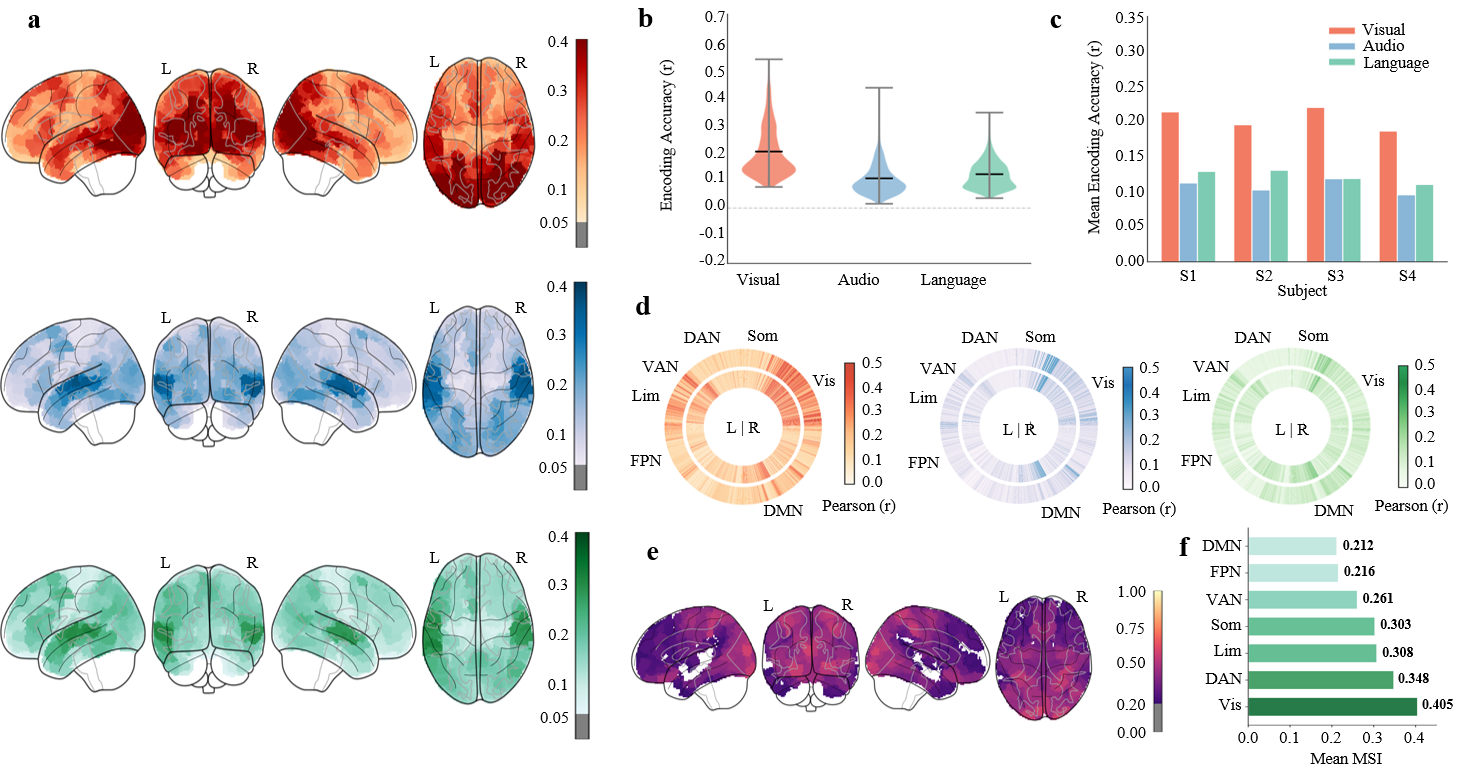
\includegraphics[width=\textwidth]{figure1.png}
    \caption{\textbf{Unimodal encoding across modalities and brain networks.}
    \textbf{a,} Encoding strength for each modality on brain surfaces.  \textbf{b,} Violin plots of encoding correlations for visual ($r = 0.204$), audio ($r = 0.107$), and language ($r = 0.122$) features. \textbf{c,} Encoding accuracy per participant. \textbf{d,} Encoding correlations for 1,000 Schaefer parcels arranged by functional network. \textbf{e,} Modality Specificity Index (MSI): sensory cortices show high specificity ($MSI > 0.4$), while DMN shows low specificity ($MSI < 0.2$). \textbf{f,} MSI hierarchy from modality-specific to integrative processing.}
    \label{fig:Fig1}
\end{figure*}

\subsection{Hierarchical Organization with the DMN as Integration Hub}

Having established the encoding asymmetry, we next ask \textit{where} multimodal integration occurs. If integration follows a hierarchical architecture with dedicated hub regions, this could provide the structural basis for an attention allocation mechanism that operates independently of encoding strength. The Multimodal Integration Index (MII) revealed a systematic gradient: the Visual network exhibited the lowest MII while the DMN exhibited the highest ($MII = 0.744$), reflecting balanced multimodal processing (Fig.~\ref{fig:Fig2}a,b). This hierarchy was consistent across participants (ICC = 0.89) and aligned with the known unimodal-to-transmodal cortical gradient \cite{margulies2016situating}. Hierarchical clustering of brain regions based on multimodal encoding profiles confirmed that regions grouped according to canonical functional networks (Fig.~\ref{fig:Fig2}c), and the network-level encoding similarity matrix showed strong within-network correlations (mean $r = 0.72$) exceeding between-network correlations (mean $r = 0.34$; $t = 15.6$, $p < 0.001$; Fig.~\ref{fig:Fig2}d).

\subsection{The Encoding-Attention Dissociation}

Sections~III-A and III-B established two prerequisites: (1)~a strong encoding asymmetry favoring vision, and (2)~a hierarchical integration architecture with the DMN as hub. We now test the central question: does the brain's attention allocation track this encoding asymmetry? If the brain followed an ``efficient'' feature-tracking strategy, attention weights should be proportional to encoding accuracy. Given visual features' $\sim$2$\times$ encoding advantage, an efficient allocation would assign approximately 47\% to visual, 28\% to language, and 25\% to audio. However, the learned attention weights from our multimodal network revealed a strikingly different pattern.

Table~\ref{tab:attn_per_subject} presents the per-subject attention weights. All four participants exhibited nearly identical balanced weights ($\sim$33\% per modality), with cross-subject standard deviations below 0.002 for each modality. The models converged via early stopping between epochs 11--13, and achieved meaningful encoding performance on the validation set (mean $r$ = 0.117--0.138, with 480--618 regions exceeding $r > 0.1$), confirming that the learned weights reflect genuine stimulus--brain relationships rather than noise.

Table~\ref{tab:dissociation} summarizes the Encoding-Attention Dissociation at the group level. The Efficiency Gap for visual was $+14.8\%$, meaning the brain under-weights its strongest modality by nearly one-third relative to what proportional allocation would predict. Conversely, audio and language are over-weighted by 9.8\% and 5.0\%, respectively.

\begin{table}[t]
\caption{Per-Subject Attention Weights from the Multimodal Network}
\label{tab:attn_per_subject}
\centering
\begin{tabular*}{\columnwidth}{@{\extracolsep{\fill}}lcccccc@{}}
\toprule
 & \multicolumn{3}{c}{Attention Weight $\alpha$} & \multicolumn{2}{c}{Val.\ Performance} \\
\cmidrule(lr){2-4} \cmidrule(lr){5-6}
Subject & Visual & Audio & Lang. & Mean $r$ & $r\!>\!0.1$ \\
\midrule
Sub-01 & 0.324 & 0.343 & 0.333 & 0.138 & 618 \\
Sub-02 & 0.321 & 0.347 & 0.331 & 0.128 & 554 \\
Sub-03 & 0.325 & 0.346 & 0.329 & 0.138 & 538 \\
Sub-05 & 0.323 & 0.347 & 0.331 & 0.117 & 480 \\
\midrule
Mean & 0.323 & 0.346 & 0.331 & 0.130 & 548 \\
SD & 0.001 & 0.002 & 0.001 & --- & --- \\
\bottomrule
\end{tabular*}
\end{table}

\begin{table}[t]
\caption{Encoding-Attention Dissociation (Group-Level Summary)}
\label{tab:dissociation}
\centering
\setlength{\tabcolsep}{8pt}
\begin{tabular}{lccc}
\toprule
 & Visual & Audio & Language \\
\midrule
Encoding $r$ & \textbf{0.204} & 0.107 & 0.122 \\
Efficient $\alpha$ & 47.1\% & 24.7\% & 28.2\% \\
Observed $\alpha$ & 32.3\% & 34.6\% & 33.1\% \\
Efficiency Gap & $+$14.8\% & $-$9.8\% & $-$5.0\% \\
\bottomrule
\end{tabular}
\end{table}

\begin{figure*}[t]
    \centering
    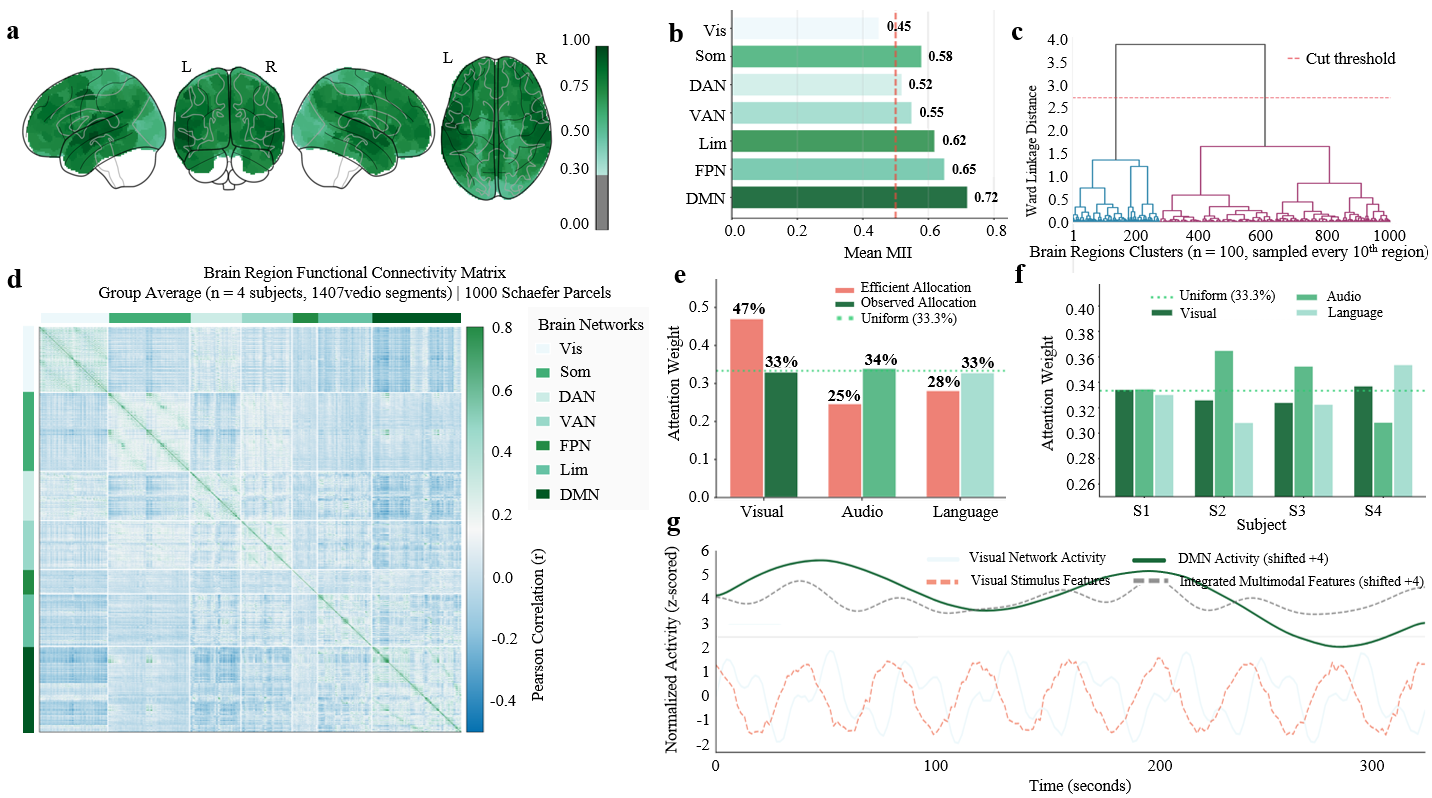
\includegraphics[width=\textwidth]{figure2.png}
    \caption{\textbf{Hierarchical integration and Encoding-Attention Dissociation.}
    \textbf{a,} MII across cortex: highest in medial prefrontal and posterior cingulate (DMN core). \textbf{b,} MII hierarchy across networks. \textbf{c,} Hierarchical clustering of 1,000 brain regions by encoding profiles. \textbf{d,} Network encoding similarity matrix. \textbf{e,} Predicted (efficient) vs.\ observed attention weights. \textbf{f,} Attention weights across participants. \textbf{g,} Temporal dynamics: Visual network tracks rapid fluctuations; DMN exhibits integrated dynamics.}
    \label{fig:Fig2}
\end{figure*}

\subsection{Control Analyses}\label{sec:controls}

The dissociation established in Section~III-C is striking, but could it arise from methodological artifacts rather than a genuine neural phenomenon? Three alternative explanations must be addressed: (1)~the multimodal model fits poorly, so weights default to uniform; (2)~the training procedure constrains weights to remain balanced; (3)~the encoding asymmetry is specific to the chosen feature models, not the modalities themselves. We conducted a targeted control analysis for each.

\subsubsection{High-Encoding Subset Analysis}
If balanced weights merely reflect poor model fit---i.e., the network fails to learn meaningful modality distinctions because predictions are too noisy---then restricting analysis to well-predicted brain regions should alter the pattern. We retrained the multimodal network three times, each time including only brain regions where the best unimodal encoding exceeded a threshold: $r > 0.1$, $r > 0.15$, and $r > 0.2$.

Table~\ref{tab:subset_detail} presents per-subject results at each threshold. Even at the strictest threshold ($r > 0.2$), which retains only 333--465 of 1,000 regions per subject, the attention weights remained balanced. Strikingly, the weights became \textit{more} balanced at higher thresholds (Fig.~\ref{fig:Fig3}a): the coefficient of variation (CV) of the three modality weights decreased from 0.036 at $r > 0.1$ to 0.011 at $r > 0.2$. This means the dissociation is strongest precisely in the brain regions where encoding models perform best, directly contradicting the poor-fit explanation.

\begin{table}[t]
\caption{High-Encoding Subset Analysis: Per-Subject Results}
\label{tab:subset_detail}
\centering
\begin{tabular*}{\columnwidth}{@{\extracolsep{\fill}}clcccc@{}}
\toprule
Threshold & Subject & Regions & Visual & Audio & Lang. \\
\midrule
\multirow{4}{*}{$r\!>\!0.1$}
 & Sub-01 & 944 & 0.327 & 0.344 & 0.329 \\
 & Sub-02 & 929 & 0.325 & 0.346 & 0.329 \\
 & Sub-03 & 982 & 0.325 & 0.346 & 0.330 \\
 & Sub-05 & 928 & 0.324 & 0.347 & 0.330 \\
\midrule
\multirow{4}{*}{$r\!>\!0.15$}
 & Sub-01 & 715 & 0.328 & 0.342 & 0.331 \\
 & Sub-02 & 627 & 0.326 & 0.344 & 0.330 \\
 & Sub-03 & 695 & 0.325 & 0.345 & 0.331 \\
 & Sub-05 & 549 & 0.331 & 0.337 & 0.332 \\
\midrule
\multirow{4}{*}{$r\!>\!0.2$}
 & Sub-01 & 448 & 0.333 & 0.334 & 0.334 \\
 & Sub-02 & 383 & 0.330 & 0.336 & 0.334 \\
 & Sub-03 & 465 & 0.327 & 0.337 & 0.336 \\
 & Sub-05 & 333 & 0.331 & 0.336 & 0.333 \\
\bottomrule
\end{tabular*}
\end{table}

\subsubsection{End-to-End Training Control}
If balanced weights were an artifact of the training procedure---for example, if the learning rate were too high for the modality weights to differentiate---then changing the training configuration should alter the result. We retrained the full model for all four subjects using a lower learning rate ($5 \times 10^{-5}$, halved from the standard $10^{-4}$), allowing finer-grained gradient updates to the modality weight parameters. As shown in Table~\ref{tab:e2e_detail}, the resulting weights remained balanced across all subjects (mean: V = 0.328, A = 0.343, L = 0.329), confirming that the finding is not sensitive to training hyperparameters.

\begin{table}[t]
\caption{End-to-End Training Control (lr = $5 \times 10^{-5}$)}
\label{tab:e2e_detail}
\centering
\begin{tabular*}{\columnwidth}{@{\extracolsep{\fill}}lcccc@{}}
\toprule
Subject & Visual & Audio & Language & Val.\ $r$ \\
\midrule
Sub-01 & 0.329 & 0.342 & 0.329 & 0.137 \\
Sub-02 & 0.326 & 0.344 & 0.330 & 0.128 \\
Sub-03 & 0.329 & 0.342 & 0.329 & 0.128 \\
Sub-05 & 0.327 & 0.345 & 0.329 & 0.100 \\
\midrule
Mean & 0.328 & 0.343 & 0.329 & 0.123 \\
\bottomrule
\end{tabular*}
\end{table}

\subsubsection{Multi-Model Feature Robustness}\label{sec:multimodel}
A critical concern is whether our findings reflect properties of the specific feature extraction models rather than properties of the modalities themselves. If, for example, SlowFast happens to produce unusually brain-predictive features while MFCC features are unusually poor, the apparent visual dominance could be a model artifact rather than a modality-level phenomenon.

To address this, we extracted features using an entirely independent set of models: CLIP ViT-B/32 \cite{radford2021learning} for visual features (768D, pretrained on image-text pairs), Wav2Vec2-base \cite{baevski2020wav2vec} for audio (768D, self-supervised speech representations), and GPT-2 \cite{radford2019language} for language (768D, autoregressive language model). These models differ fundamentally from the primary models in architecture (transformer vs.\ CNN, self-supervised vs.\ supervised), training data, and output dimensionality.

Table~\ref{tab:multimodel_detail} and Fig.~\ref{fig:Fig3}b show per-subject encoding results for both feature sets. Despite these differences, the modality ordering was preserved in every subject: visual encoding consistently produced the highest correlation, followed by language, then audio. The visual-to-audio encoding ratio was 1.9$\times$ with primary models and 1.4$\times$ with alternative models---different in magnitude but consistent in direction. This confirms that visual encoding dominance is a property of the sensory modality during naturalistic movie viewing, not an artifact of any specific feature extraction model. Fig.~\ref{fig:Fig3}c visualizes the dissociation directly: under efficient allocation, each point (one per subject $\times$ modality) would fall on the diagonal; instead, all points cluster near the horizontal uniform line.

\begin{table}[t]
\caption{Multi-Model Encoding: Per-Subject Comparison}
\label{tab:multimodel_detail}
\centering
\begin{tabular*}{\columnwidth}{@{\extracolsep{\fill}}llcccc@{}}
\toprule
Modality & Model & S01 & S02 & S03 & S05 \\
\midrule
\multirow{2}{*}{Visual}
 & SlowFast & \textbf{0.214} & \textbf{0.195} & \textbf{0.220} & \textbf{0.186} \\
 & CLIP & \textbf{0.134} & \textbf{0.129} & \textbf{0.144} & \textbf{0.123} \\
\midrule
\multirow{2}{*}{Audio}
 & MFCC & 0.112 & 0.102 & 0.118 & 0.095 \\
 & Wav2Vec2 & 0.098 & 0.098 & 0.104 & 0.089 \\
\midrule
\multirow{2}{*}{Language}
 & BERT & 0.129 & 0.130 & 0.119 & 0.110 \\
 & GPT-2 & 0.128 & 0.131 & 0.133 & 0.110 \\
\bottomrule
\end{tabular*}
\end{table}

\begin{figure*}[t]
    \centering
    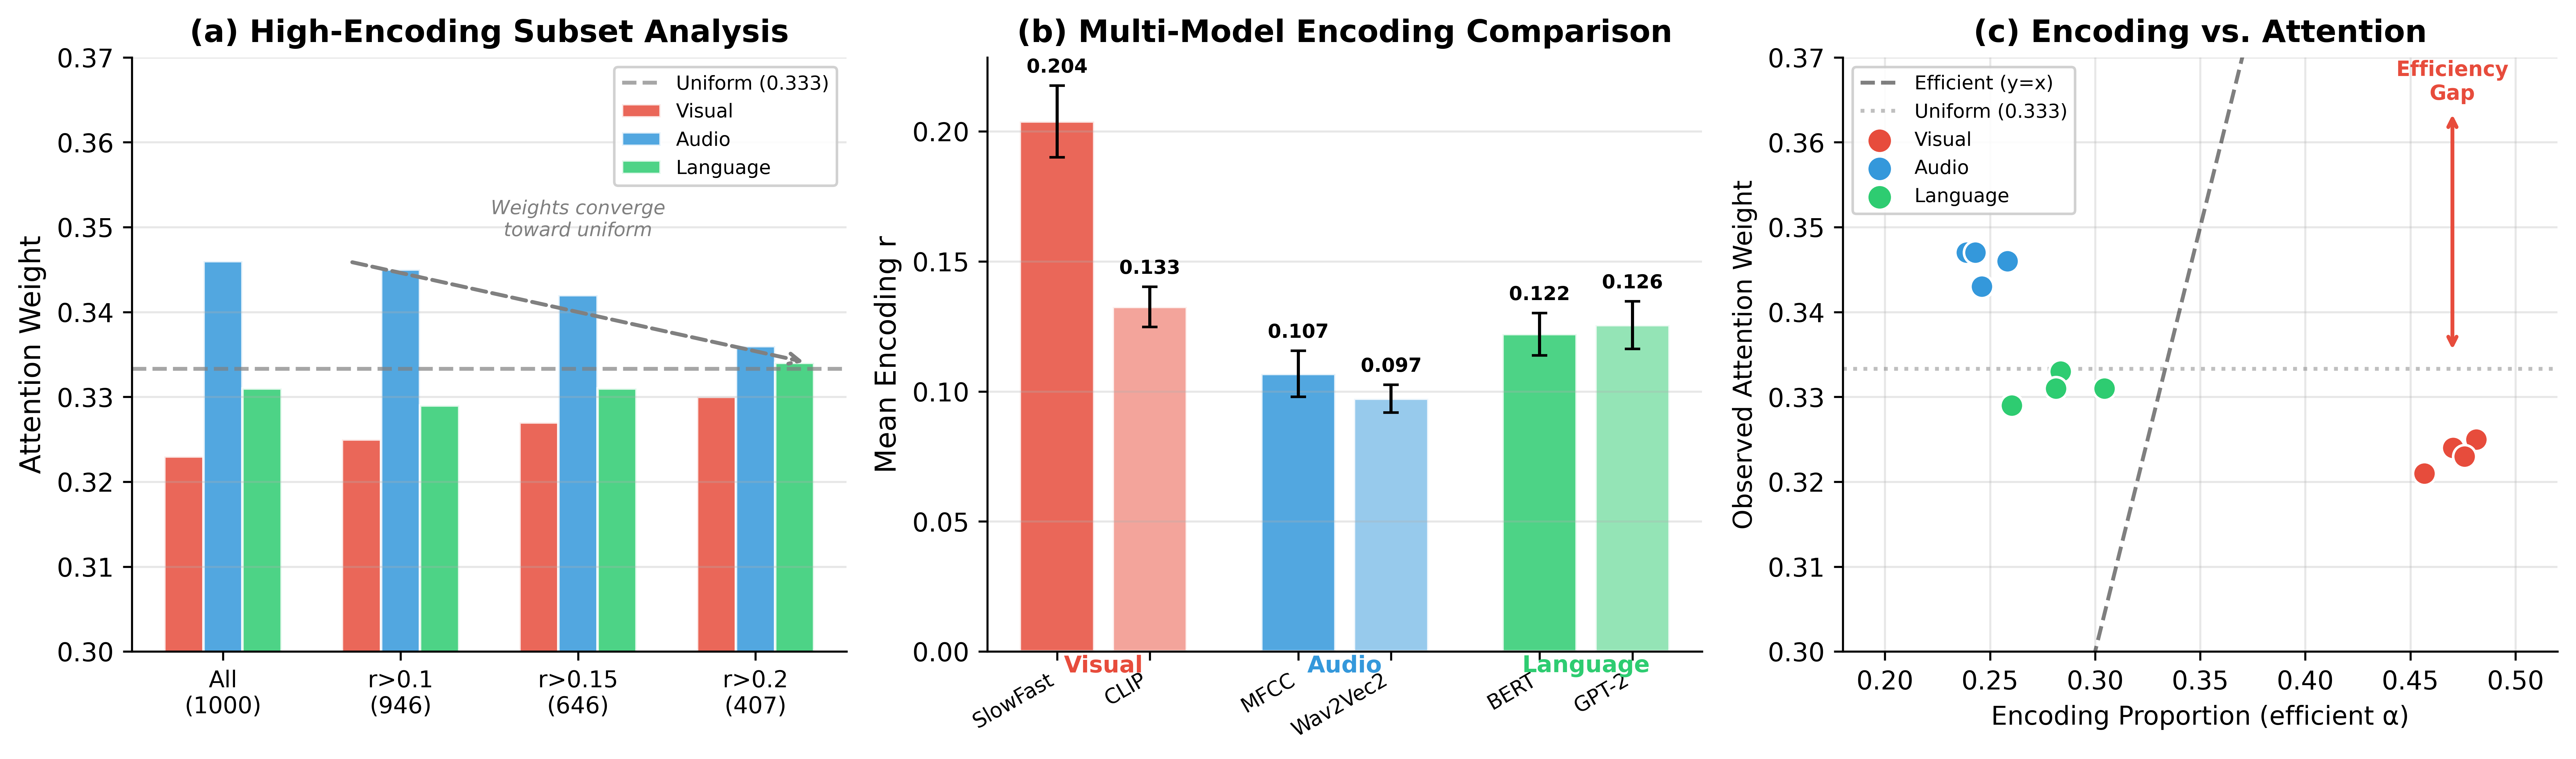
\includegraphics[width=\textwidth]{figure3_control_analyses.png}
    \caption{\textbf{Control analyses and multi-model validation.}
    \textbf{(a)} High-encoding subset analysis: attention weights across four encoding thresholds. As the threshold increases (retaining fewer, better-predicted regions), weights converge toward the uniform distribution (dashed line), demonstrating that balanced attention is strongest in well-encoded regions.
    \textbf{(b)} Multi-model encoding comparison: mean encoding correlation ($\pm$ SD across subjects) for primary models (SlowFast, MFCC, BERT) and alternative models (CLIP, Wav2Vec2, GPT-2). The Visual $>$ Language $>$ Audio ordering is preserved across both model sets.
    \textbf{(c)} Encoding proportion vs.\ observed attention weight for each subject $\times$ modality combination. Under efficient allocation, points would fall on the diagonal (dashed). Instead, all points cluster near the uniform line ($\alpha = 0.333$), visualizing the Encoding-Attention Dissociation. The ``Efficiency Gap'' for visual (red) is largest.}
    \label{fig:Fig3}
\end{figure*}

\subsection{Summary of Control Analyses}

Table~\ref{tab:controls_summary} synthesizes all conditions tested. Each row corresponds to a different potential confound: poor model fit (subset rows), training artifacts (E2E row), or model-specific effects (addressed by Table~\ref{tab:multimodel_detail}). In every case, attention weights remain within 1--2\% of the uniform distribution ($\frac{1}{3} \approx 0.333$). The maximum deviation across all 20 subject$\times$condition measurements was 2.3\%. Having ruled out the three most plausible alternative explanations, we conclude that the Encoding-Attention Dissociation reflects a genuine property of the brain's multimodal integration strategy.

\begin{table}[t]
\caption{Summary: Attention Weights Across All Conditions (Mean $\pm$ SD)}
\label{tab:controls_summary}
\centering
\begin{tabular*}{\columnwidth}{@{\extracolsep{\fill}}lccc@{}}
\toprule
Condition & Visual & Audio & Language \\
\midrule
Standard & $0.323 \pm 0.001$ & $0.346 \pm 0.002$ & $0.331 \pm 0.001$ \\
Subset $r\!>\!0.1$ & $0.325 \pm 0.001$ & $0.345 \pm 0.001$ & $0.329 \pm 0.001$ \\
Subset $r\!>\!0.15$ & $0.327 \pm 0.002$ & $0.342 \pm 0.003$ & $0.331 \pm 0.001$ \\
Subset $r\!>\!0.2$ & $0.330 \pm 0.002$ & $0.336 \pm 0.001$ & $0.334 \pm 0.001$ \\
E2E (lr=$5\!\times\!10^{-5}$) & $0.328 \pm 0.001$ & $0.343 \pm 0.001$ & $0.329 \pm 0.001$ \\
\midrule
Uniform ref. & 0.333 & 0.333 & 0.333 \\
\bottomrule
\end{tabular*}
\end{table}

\subsection{Temporal Dynamics Support Hierarchical Processing}

The previous sections established \textit{what} the brain does (balanced attention) and ruled out artifacts. We now provide evidence for \textit{how}: analysis of temporal dynamics offered additional support for the hierarchical architecture. Visual network activity closely tracked rapid fluctuations in visual features, while DMN activity exhibited slower, integrated dynamics with temporal smoothing across modalities (Fig.~\ref{fig:Fig2}g). This temporal dissociation is consistent with the hierarchical framework: fast, modality-specific processing in sensory regions feeds into slower, integrated processing in association cortex. The DMN's temporal smoothing may reflect the mechanism by which balanced attention is maintained---by operating on temporally integrated representations rather than raw stimulus features, the DMN can implement attention allocation that is decoupled from moment-to-moment fluctuations in modality strength.

\section{Discussion}

\subsection{The Encoding-Attention Dissociation Challenges Bayesian Optimality}

Our results support all three hypotheses and, through extensive control analyses, establish the Encoding-Attention Dissociation as a robust phenomenon. The central finding---that attention weights remain balanced at $\sim$33\% per modality despite a twofold visual encoding advantage---challenges the classical Bayesian framework predicting that attention tracks signal reliability \cite{ernst2002humans, knill2004bayesian}.

This dissociation is consistent with theoretical perspectives emphasizing ecological rationality \cite{gigerenzer2009homo}: in naturalistic settings where modality informativeness varies unpredictably across scenes, balanced attention may hedge against uncertainty, prioritizing robustness over narrow efficiency. A movie scene that is visually uninformative (e.g., a dark screen during dialogue) but aurally rich would suffer under a visual-dominant attention strategy. By maintaining balanced attention regardless of average encoding strength, the brain ensures reliable multimodal processing across the full range of naturalistic conditions.

\subsection{Validity of Learned Weights as Attention Proxies}

The interpretation of the learned modality weights as proxies for neural attention allocation is supported by three converging observations. First, the model achieves meaningful prediction performance across 480--618 brain regions per subject ($r > 0.1$), indicating that the stimulus--brain relationships captured are non-trivial \cite{kriegeskorte2008representational, yamins2016using}. Second, the weights are remarkably consistent across four independent participants (SD $< 0.002$ for each modality), suggesting a stable integration principle rather than model-specific artifacts. Third, the weights systematically diverge from encoding strength predictions in the same direction for all subjects, consistent with theoretical accounts of attention as a distinct selection mechanism separate from encoding \cite{lindsay2020attention}.

\subsection{Implications of Control Analyses}

The three control analyses collectively address the most plausible alternative explanations.

The high-encoding subset analysis addresses the concern that balanced weights arise from noise in poorly predicted regions. By progressively restricting the analysis to regions with $r > 0.1$, $0.15$, and $0.2$, we showed that balanced attention not only persists but \textit{intensifies} (CV decreasing from 0.036 to 0.011). This counterintuitive finding suggests that the dissociation is a feature of how the brain integrates well-encoded information, not an artifact of encoding failure.

The end-to-end training control addresses the concern that the training procedure artificially constrains the weights. By halving the learning rate, we allowed finer-grained optimization of the modality weights while maintaining the same architecture. The weights remained balanced (V = 0.328, A = 0.343, L = 0.329), confirming that the uniform distribution is not an artifact of learning dynamics.

The multi-model analysis addresses the fundamental question of whether our claims are about modalities or about specific feature extraction models. Using CLIP \cite{radford2021learning} (vision transformer trained on image-text pairs), Wav2Vec2 \cite{baevski2020wav2vec} (self-supervised speech model), and GPT-2 \cite{radford2019language} (autoregressive language model)---architectures that differ from the primary models in every major design choice---we confirmed that the visual $>$ language $>$ audio encoding ordering is preserved. This validates that the encoding dominance pattern is a property of how the brain processes different sensory modalities during naturalistic movie viewing, not an artifact of any particular computational model.

\subsection{Hierarchical Integration Architecture}

Beyond the attention allocation finding, our results confirm that multimodal integration follows a hierarchical architecture with the DMN as the primary hub. The systematic MII gradient from Visual network (lowest) to DMN (highest, MII = 0.744) aligns with the known unimodal-to-transmodal cortical gradient \cite{margulies2016situating} and extends it by demonstrating that this gradient governs multimodal attention allocation, not just representational content. The DMN's role as an integration hub is consistent with its established function in narrative comprehension \cite{simony2016dynamic} and suggests that the balanced attention strategy may be architecturally enabled by the DMN's position atop the cortical hierarchy---operating on already-abstracted representations rather than raw sensory features.

\subsection{Limitations}

Several limitations should be acknowledged. Our sample size ($n = 4$) limits generalizability, though high cross-subject consistency (ICC = 0.89) and the replication across multiple control conditions provides confidence. The naturalistic movie stimuli, while ecologically valid, confound multiple factors---the observed visual dominance may partly reflect the films' visual richness rather than a universal property of multimodal processing. The correlational nature of the analysis precludes causal conclusions about whether the hierarchical architecture causes the Encoding-Attention Dissociation. The attention weights, while validated through multiple controls, remain an indirect proxy derived from a computational model; future work incorporating direct neural manipulations (e.g., TMS to the DMN) or behavioral attention measures would strengthen the mechanistic account. Finally, the alternative feature models, while architecturally distinct, all represent deep learning approaches; incorporating classical signal-processing features (e.g., Gabor filters for vision) could further strengthen the multi-model validation.

\section{Conclusion}

This study provides evidence for an Encoding-Attention Dissociation in the brain's multimodal processing: despite visual features dominating encoding in 91\% of cortical regions, attention weights remain balanced at approximately 33\% per modality. Through control analyses spanning encoding thresholds, training strategies, and feature extraction models, we demonstrate that this finding is robust and reflects a genuine property of multimodal integration rather than a methodological artifact. The DMN serves as the primary integration hub within a hierarchical framework ascending from modality-specific sensory cortex. Together, these findings suggest that the brain's apparent inefficiency in attention allocation may reflect an optimization for robustness---maintaining balanced integration regardless of encoding strength to ensure reliable multimodal processing across diverse naturalistic contexts.

\section{Data and Code Availability}

The fMRI data are available through the Algonauts Project 2025 Challenge (\url{https://algonautsproject.com/}). Analysis code will be made publicly available upon publication.

\section*{Acknowledgment}

This work used data from the Courtois NeuroMod project and the Algonauts 2025 Challenge.

\begin{thebibliography}{00}
\bibitem{stein1993merging} B.~E. Stein and M.~A. Meredith, \textit{The Merging of the Senses}. MIT Press, 1993.
\bibitem{beauchamp2004unraveling} M.~S. Beauchamp \textit{et al.}, ``Unraveling multisensory integration: patchy organization within human STS multisensory cortex,'' \textit{Nature Neuroscience}, vol.~7, no.~11, pp.~1190--1192, 2004.
\bibitem{ernst2002humans} M.~O. Ernst and M.~S. Banks, ``Humans integrate visual and haptic information in a statistically optimal fashion,'' \textit{Nature}, vol.~415, no.~6870, pp.~429--433, 2002.
\bibitem{knill2004bayesian} D.~C. Knill and A.~Pouget, ``The Bayesian brain: the role of uncertainty in neural coding and computation,'' \textit{Trends in Neurosciences}, vol.~27, no.~12, pp.~712--719, 2004.
\bibitem{fetsch2013bridging} C.~R. Fetsch, G.~C. DeAngelis, and D.~E. Angelaki, ``Bridging the gap between theories of sensory cue integration and the physiology of multisensory neurons,'' \textit{Nature Reviews Neuroscience}, vol.~14, no.~6, pp.~429--442, 2013.
\bibitem{mishra2012attention} J.~Mishra and A.~Gazzaley, ``Attention distributed across sensory modalities enhances perceptual performance,'' \textit{J.~Neuroscience}, vol.~32, no.~35, pp.~12294--12302, 2012.
\bibitem{naselaris2011encoding} T.~Naselaris \textit{et al.}, ``Encoding and decoding in fMRI,'' \textit{NeuroImage}, vol.~56, no.~2, pp.~400--410, 2011.
\bibitem{gucclu2015deep} U.~G{\"u}{\c{c}}l{\"u} and M.~A.~J. van Gerven, ``Deep neural networks reveal a gradient in the complexity of neural representations across the ventral stream,'' \textit{J.~Neuroscience}, vol.~35, no.~27, pp.~10005--10014, 2015.
\bibitem{huth2016natural} A.~G. Huth \textit{et al.}, ``Natural speech reveals the semantic maps that tile human cerebral cortex,'' \textit{Nature}, vol.~532, no.~7600, pp.~453--458, 2016.
\bibitem{caucheteux2022brains} C.~Caucheteux and J.-R. King, ``Brains and algorithms partially converge in natural language processing,'' \textit{Communications Biology}, vol.~5, no.~1, p.~134, 2022.
\bibitem{margulies2016situating} D.~S. Margulies \textit{et al.}, ``Situating the default-mode network along a principal gradient of macroscale cortical organization,'' \textit{Proc.~Natl.~Acad.~Sci.}, vol.~113, no.~44, pp.~12574--12579, 2016.
\bibitem{schaefer2018local} A.~Schaefer \textit{et al.}, ``Local-global parcellation of the human cerebral cortex from intrinsic functional connectivity MRI,'' \textit{Cerebral Cortex}, vol.~28, no.~9, pp.~3095--3114, 2018.
\bibitem{mar2011neural} R.~A. Mar, ``The neural bases of social cognition and story comprehension,'' \textit{Ann.~Rev.~Psychology}, vol.~62, no.~1, pp.~103--134, 2011.
\bibitem{simony2016dynamic} E.~Simony \textit{et al.}, ``Dynamic reconfiguration of the default mode network during narrative comprehension,'' \textit{Nature Communications}, vol.~7, no.~1, p.~12141, 2016.
\bibitem{feichtenhofer2019slowfast} C.~Feichtenhofer \textit{et al.}, ``SlowFast networks for video recognition,'' in \textit{Proc.~IEEE/CVF ICCV}, 2019, pp.~6202--6211.
\bibitem{devlin2019bert} J.~Devlin \textit{et al.}, ``BERT: Pre-training of deep bidirectional transformers for language understanding,'' in \textit{Proc.~NAACL-HLT}, 2019, pp.~4171--4186.
\bibitem{vaswani2017attention} A.~Vaswani \textit{et al.}, ``Attention is all you need,'' \textit{Advances in Neural Information Processing Systems}, vol.~30, 2017.
\bibitem{desimone1984stimulus} R.~Desimone \textit{et al.}, ``Stimulus-selective properties of inferior temporal neurons in the macaque,'' \textit{J.~Neuroscience}, vol.~4, no.~8, pp.~2051--2062, 1984.
\bibitem{gigerenzer2009homo} G.~Gigerenzer and H.~Brighton, ``Homo heuristicus: Why biased minds make better inferences,'' \textit{Topics in Cognitive Science}, vol.~1, no.~1, pp.~107--143, 2009.
\bibitem{lindsay2020attention} G.~W. Lindsay, ``Attention in psychology, neuroscience, and machine learning,'' \textit{Frontiers in Computational Neuroscience}, vol.~14, p.~29, 2020.
\bibitem{shrout1979intraclass} P.~E. Shrout and J.~L. Fleiss, ``Intraclass correlations: uses in assessing rater reliability,'' \textit{Psychological Bulletin}, vol.~86, no.~2, p.~420, 1979.
\bibitem{gifford2024algonauts} A.~T. Gifford \textit{et al.}, ``The Algonauts project 2025 challenge: How the human brain makes sense of multimodal movies,'' \textit{arXiv:2501.00504}, 2024.
\bibitem{boyle2023courtois} J.~Boyle \textit{et al.}, ``The Courtois NeuroMod project: quality assessment of the initial data release,'' in \textit{Conf.~Cognitive Computational Neuroscience}, 2023.
\bibitem{kriegeskorte2008representational} N.~Kriegeskorte, M.~Mur, and P.~A. Bandettini, ``Representational similarity analysis---connecting the branches of systems neuroscience,'' \textit{Frontiers in Systems Neuroscience}, vol.~2, p.~249, 2008.
\bibitem{yamins2016using} D.~L.~K. Yamins and J.~J. DiCarlo, ``Using goal-driven deep learning models to understand sensory cortex,'' \textit{Nature Neuroscience}, vol.~19, no.~3, pp.~356--365, 2016.
\bibitem{radford2021learning} A.~Radford \textit{et al.}, ``Learning transferable visual models from natural language supervision,'' in \textit{Proc.~ICML}, 2021, pp.~8748--8763.
\bibitem{baevski2020wav2vec} A.~Baevski \textit{et al.}, ``wav2vec 2.0: A framework for self-supervised learning of speech representations,'' in \textit{Advances in Neural Information Processing Systems}, vol.~33, 2020, pp.~12449--12460.
\bibitem{radford2019language} A.~Radford \textit{et al.}, ``Language models are unsupervised multitask learners,'' \textit{OpenAI Blog}, vol.~1, no.~8, p.~9, 2019.
\end{thebibliography}

\end{document}
